%%%%%%%%%%%%%%%%%%%%%%% file typeinst.tex %%%%%%%%%%%%%%%%%%%%%%%%%
%
% This is the LaTeX source for the instructions to authors using%
% the LaTeX document class 'llncs.cls' for contributions to
% the Lecture Notes in Computer Sciences series.
% http://www.springer.com/lncs       Springer Heidelberg 2006/05/04
%
% It may be used as a template for your own input - copy it
% to a new file with a new name and use it as the basis
% for your article.
%
% NB: the document class 'llncs' has its own and detailed documentation, see
% ftp://ftp.springer.de/data/pubftp/pub/tex/latex/llncs/latex2e/llncsdoc.pdf
%
%%%%%%%%%%%%%%%%%%%%%%%%%%%%%%%%%%%%%%%%%%%%%%%%%%%%%%%%%%%%%%%%%%%
\documentclass[runningheads,a4paper]{llncs}
%%nachträglich hinzugefügt:
\usepackage[utf8]{inputenc}
%%
%packet für python code highlighting
%\usepackage{minted}
%\definecolor{bg}{rgb}{0.95,0.95,0.95}

\usepackage{amssymb}
\setcounter{tocdepth}{3}
\usepackage{graphicx}

%tabelle
\usepackage{rotating}
\usepackage{booktabs}
\usepackage{multirow}

%einige Mathefunktionen
\usepackage{amsmath}

%Für Codelistings
\usepackage{listings}

%was ist das?
\usepackage{float}
%\usepackage{capt-of}

\usepackage{url}
\urldef{\mailsa}\path|{marcus.voss, eric.weissbrich}@student.hu-berlin.de|    
\newcommand{\keywords}[1]{\par\addvspace\baselineskip
\noindent\keywordname\enspace\ignorespaces#1}

%%empfohleneder bibliography style
\bibliographystyle{splncs03}

\begin{document}
%Abstand zwischen den Absätzen.
\setlength{\parskip}{3.5pt}

\mainmatter  % start of an individual contribution

% first the title is needed
\title{Readability Analysis of Privacy Policies}

% a short form should be given in case it is too long for the running head
\titlerunning{Readability Analysis of Privacy Policies}

% the name(s) of the author(s) follow(s) next
%
% NB: Chinese authors should write their first names(s) in front of
% their surnames. This ensures that the names appear correctly in
% the running heads and the author index.
%
\author{Marcus Voss
%\thanks{Please note that the LNCS Editorial assumes that all authors have used
%the western naming convention, with given names preceding surnames. This determines
%the structure of the names in the running heads and the author index.}%
\and Eric Lee Weißbrich}
%
\authorrunning{Readability Analysis of Privacy Policies   }
% (feature abused for this document to repeat the title also on left hand pages)

% the affiliations are given next; don't give your e-mail address
% unless you accept that it will be published
\institute{%\mailsa\\
Humboldt Universität zu Berlin,\\ 
Institute of Information Systems\\
\mailsa\\
%\mailsb\\
%\mailsc\\
%\url{http://www.springer.com/lncs}
}

%
% NB: a more complex sample for affiliations and the mapping to the
% corresponding authors can be found in the file "llncs.dem"
% (search for the string "\mainmatter" where a contribution starts).
% "llncs.dem" accompanies the document class "llncs.cls".
%

\toctitle{Lecture Notes in Computer Science}
\tocauthor{Authors' Instructions}
\maketitle


\begin{abstract}
Generally the internet user is not aware about how his personal data is collected, used and disclosed by internet services he uses, because he doesn't read their privacy policies. Assuming that the readability of a policy influences this behavior, we develop tool Privacy Policy Analyzer, which is used to analyze privacy policies based on different measures for text difficulty. We provide an overview over the common classic readability measures as well as state of the art approaches and work for visualization. We show that the readability level of the privacy policies from the most popular web sites is at college level or above. In coherence with the average age of the internet user and their education, one essential statement is, that in general privacy policies are to difficult, when compared to the reading comprehension level of the average internet user. An improvement of readability is necessary to cover most internet users and give them a chance of understanding privacy policies easily. Using Google as an example we show that an improvement of readability can be achieved.

\keywords{Readability, Privacy Policies, NLTK}
\end{abstract}

\section{Introduction}
\subsection{Motivation}
The control over personal information in the internet becomes an increasing need. Users disclose more and more information while using internet services on a daily basis without knowing how information is collected, used and disclosed by the service provider. Privacy policies do explain how the data provided by the user is processed.

Although most people do care about privacy and how their personal information is used on the internet, they do generally not read privacy policies - not even of the websites they are using most frequently \cite{Singleton2001}. By doing so they could improve awareness regarding their privacy in the internet.

One assumption could be that the fact that few people are actually reading privacy policies depends on their \emph{readability}. In this paper we will therefore implement a tool to analyze and compare the readability levels required to comfortably read privacy policies of popular web sites. The precise research question will follow in section \ref{sec:researchquestion}.

To cover the aspects of the research topic regarding privacy policies the paper is organized as follows: The theoretical part \ref{sec:theory} first covers related work in this field. We will then give an overview over various established measures in section \ref{sec:readability_measures} and continue with recent work in the field of readability and the visualization of text difficulty. After these theoretical foundations our proposed practical approach is described in section \ref{sec:method} by starting with python and the frameworks that are used. We continue to describe how we transferred the theoretical foundations into a working program that delivers specific results with strong focus on the visualization of readability in section \ref{sec:visualization}. As a result the detailed analysis of exemplary sites follows directly in section \ref{sec:results}.
Finally we deliver a conclusion, including topics fore future work and existing research limitations to our approach \ref{sec:conclusion}.


\subsection{Research question}\label{sec:researchquestion}
The goal of this paper is to analyze popular sites privacy policies by developing a tool based on different measures for text difficulty.
The tool should facilitate the readability analysis a policy and provide for comparison between different company's privacy policies. 
It will further enable the evaluation of the discrepancy between the difficulty to read a policy and the reading comprehension level of the average internet user.

\section{Theory}\label{sec:theory}
\subsection{Related Work}\label{sec:relatedwork}
%Here most important: \cite{Sumeeth2010}, but see also \cite{Singh2011}
%Not published: \cite{Huning2010}

In their paper "Are Online Privacy Policies Readable?" from 2010, Summeeth et al.\cite{Sumeeth2010} elaborate a similar research question. After explaining the requirements and restrictions of privacy policies in general they define specific requirements (e.g. structure, content, accessibility) that make these policies readable. They collect a selection of privacy policies from popular internet sites and analyze their readability with the aid of readability formulas. For the analysis Sumeeth et al. use various classic measures such as the Flesh Readability Score, Dale-Chall Index, Fog Index, Fry Graph and few others. After the general analysis they compare the given results with those of Hochhauser \cite{hochhauser2002}, Anton et al. \cite{Anton2004} and Jensen and Potts \cite{Jensen2004} and come to the conclusion that privacy policies are getting shorter over time and that on average a reading comprehension at college level (grade levels of 12-14) is required to understand the policies. This is lower than the average education level of the internet user and U.S. population today. The general statement of the paper is that policies getting more and more readable, but that a certain awareness of the providers needs to be maintained to further keep and improve the accessibility and readability of the policies.

The unpublished paper from Huning, "Readability of Privacy Policies of German Websites - Are users able to understand what they agree on?" \cite{Huning2010} has the main focus on a differentiation between German and English policies. It analyses various German privacy policies with the German Flesch Readability Score, the Lix and the Wiener Sachtextformel. The paper provides a basic overview over the readability, but the results are limited by the fact that the measures applied are not necessarily comparable among different languages.

Another relating publication is "A Comparative Study of Online Privacy Policies and Formats" by McDonald et al. \cite{Mcdonald2009}. They compare three different approaches of privacy policy formats to improve their readability. The first approach is to derive a shortened and standardized form of arbitrary privacy policies. The second is a standardization of privacy policies in a bulleted format. The third and last evaluation is on the common non-standardized policy. With these three formats of notation they tested the readability with more than 700 participants and came to the result that all kinds of notations were disliked and were not easily readable for everyone.

An approach from a different point of view gives the article "How Users Read and Comprehend Privacy Policies" by Vu et al.\cite{Vu2007}. Vu et al. analyze reading habits and understanding regarding privacy policies with Eye-gaze data. The participants in the survey have to answer various questions regarding policy contents. With the Eye-gaze data Vu et al. observe how the attendees search for information in the text. The result of the study is that most attendees find it very hard to extract the relevant information out of policies because of their bad structure and incomprehensible formulation.

Agrawal et al. do not focus solely on the readability, but rather focus on the comparison regarding the content of privacy policies in their paper "Ranking Privacy Policy" \cite{Agrawal2007}. The goal is to rank different privacy policies against each other. They develop a new mathematical model to rank every policy based on content. The model analyzes the various components of the policies and provides an final score, on which one could decide how "good" or "bad" the given policy seems to be. The paper however only analyzes only a few exemplary sites.

\subsection{Readability measures} \label{sec:readability_measures}

The Literacy Dictionary (by Harris and Hodges 1995) defines \emph{readability} as “the ease of comprehension because of style of writing" (as found in \cite{Fry2006}). Dale and Chall give a more refined definition in 1949, by stating that readability is "the sum total (including interactions) of all those elements within a given piece of printed material that effect the success of a group of readers have with it. The success is the extend to which they understand it, read it at an optimal speed, and find it interesting" as found in \cite{Chall1995}).

\emph{Readability formulas} are an attempt to make assessing readability of texts objective - most are even so objective that they can be automated. A readability formula is an equation which combines different text features that best predict text difficulty \cite{Chall1995}. 

The development of such an equation is done by studying the relationship between different text features and readability. The proof of success of a readability formulas is a correlation with the score obtained by a reading comprehension test applied to texts of different difficulties (so called criterion passages). Those comprehension tests can be a multiple choice tests assessing the readers understanding, also the so called Cloze Test (see below), or expert rating of the the difficulty. Also concurrent validity - that is the analysis of correlation with another reading measure - is a common method to verify a formula \cite{Fry2006}.

The Cloze Test was proposed by Taylor in 1953 \cite{Taylor1953} when he wanted to oppose the then widely used readability formulas. He reasoned that text difficulty was rather influenced by the relationship among words and not by the words on itself. So he proposed a deletion test, where words of a passage where randomly deleted and had to be filled in by the reader. The amount of words that can be deleted without influencing the readers understanding than influences the final Cloze Score. However, this test can by its nature not be used instead of the formulas, since it is relying on a large panel of testing readers. By giving a better alternative to the then widely used multiple choice tests it does still however have a big influence on readability measures as it is widely used for testing the correlation of readability formulas \cite{Chall1995}.

Most readability formulas are based on two different kinds of inputs that have been verified as the text features best predicting a text's readability by most of the research studies:
\begin{enumerate}
	\item measures based on syntactic difficulty,
	\item measures based on semantic difficulty.
\end{enumerate}
The first refers to the grammatical complexity and is in most formulas measured by the sentence length (e.g. average words per sentence). This rather simple metric functions quite well as a predictor, even when compared to more complex syntactic measures \cite{Chall1995}.
The second refers to the meaning of the words. A common measure among many formulas is the word length (e.g. measured in syllables or number of letters in a word). Another approach is the word frequency - this can be realized by comparing the appearance of the words of the text to the frequency of the words in other pre-classified texts (see language models), or the fact that words of the text do or don't appear on a list of easy words (see Dale-Chall Readability index in \ref{sec:dale_chall}). The Bermouth Formula even combines both approaches for semantic difficulty: word length and a word list (see \cite{Chall1995}, and \cite{Fry2006}).

One of readability formula's most common usage is in education, to help students to learn to read better by finding the right book for for a student's current reading level. But besides in schools, readability has also been in interest by companies such as General Motors, as well as the U.S. Army and the U.S. Navy. In the United States readability is even required by law for insurance policies in some states. In 1984 the New York federal appellate court ruled in a case where a letter by the U.S. Department of Health was too difficult to read \cite{Fry2006}.

Below a selection of the most popular readability formulas is described regarding its history, included features and the calculation.


\subsubsection{Flesch Reading Ease}
The Flesch Reading Ease is one of the most used and tested readability measures. It was developed by Rudolf Flesch in 1949 and is based on the number of words, sentences and syllables.
The original result is a number from 0 to 100, with 0 as the most difficult and 100 the easiest readability score \cite{Dubay2004}.

 \begin{equation} FRE = 206.835 - 1.015 \cdot \frac{\text{total words}}{\text{total sentences}} - 84.6 \cdot \frac{\text{total syllables}}{\text{total words}} \end{equation}
 
 
 \subsubsection{Flesch-Kincaid Grade Level}
 
 The Flesch-Kincaid formula is a modified version of the original Flesch formula. The intention was a mapping of grade levels to the results of the Flesch reading ease. It was developed in 1976 as part of a study by the U.S. Navy \cite{Dubay2004}. The grade level can be considered as being the number of school years that someone needs to comfortably read a text (according to the American school system: e.g. 12 for 12th grade, or 13 for first year of college). This concept is used as discussed in the following by several measures.
 
 \begin{equation}FK-Grade = 0.39 \cdot \frac{\text{total words}}{\text{total sentences}} + 11.8 \cdot \frac{\text{total syllables}}{\text{total words}} - 15.59 \end{equation}

 
\subsubsection{Rate Index (RIX)}
The Rate Index (RIX)  is one of the more simple readability tests. It can not only be applied to English, but also on most of the western European languages \cite{webmining2007}.

 \begin{equation} RIX = \frac{\text{long words}}{sentences},\end{equation}
 \begin{equation*}
 \text{where long words = words where number of characters $>$ 6}
 \end{equation*}
 
 The usual result of the formula is between 0 and 55+. Where 0 is very easy and 55 or more very difficult \cite{webmining2007}.
 The RIX is based on the \emph{LIX} formula which was developed for the Swedish language.
 
 \subsubsection{Coleman Liau Index}
 
 The Coleman-Liau index (CLI) was introduced 1975. The intention of this formula is a simple mechanism to calculate the readability level without counting syllables. That means the automated generation of the CLI was quite simple and did not need any manual counting of text parts. The result from the Coleman Liau Index results into a grade level \cite{webmining2007}.

 \begin{equation} CLI = 5.89 \cdot \frac{characters}{words} - 30 \cdot \frac{sentences}{words} - 15.8 \end{equation}


\subsubsection{Gunning Fog Index}
 The Gunning Fog Index gives also results into a grade leven and also includes sentence length and word length as parameters \cite{webmining2007}. 
 
 \begin{equation} GFI = 0.4 \cdot \frac{words}{sentence} + 100 \cdot \frac{\text{complex words}}{words},  \end{equation}
 \begin{equation*}
 \text{where complex words = words with three or more syllables}
 \end{equation*}

\subsubsection{SMOG}

G. Harry McLaughlin published his SMOG formula in 1969. By counting the number of words of more than two syllables (polysyllable count) in 30 sentences, he provides this simple formula:
\begin{equation}
\text{SMOG} = 3 + \sqrt{\text{polysyllable count}}
\end{equation}
 
The SMOG formula generally predicts scores at least two grades higher than the Dale-Chall formula \cite{Dubay2004}.

\subsubsection{ARI}

Smith and Senter  created the Automated Readability Index in 1967 for the U.S. Army \cite{Dubay2004}. They used an modified electric typewriter to derive the necessary counters for words and sentences.
The ARI formula produces reading grade levels:% \cite{Smith1967}:%TODO Quelle von dir Marcus? nicht im bib enthalten

\begin{equation}
ARI = 0.50 \cdot \text{words per sentence} + 4.71 \cdot \text{strokes per word} – 21.43 
\end{equation}


\subsubsection{New Dale Chall} \label{sec:dale_chall}
%\cite{Dubay}[p. 52f.]
The Dale-Chall Readability index uses a word list of easy, "familiar" words to express the semantic difficulty. For the New Dale-Call Readability Formula, Chall and Dale updated their list of 3000 easy words in 1995 from their original formula of 1948. The 3000 words are known to 80 percent of students in 4th grade and may hence be viewed as the most elemental words in the English language. This can basically be seen as a simple language model, as here the list of 3000 words is classified as "easy" - hence a text that uses more of these words can also be seen as easy (and vice versa for "hard" words). The new formula correlates .93 with the mean Cloze Scores, making it the most valid of the popular formulas when compared to other of the classic formulas \cite{Chall1995} \cite{Dubay2007}.

\begin{equation}
\text{Raw Score} = 0.1579 \cdot PDW + 0.0496 \cdot \text{Average Sentence Length},
\end{equation}
\begin{equation*}
\text{where PDW =} \frac{\text{words not on Dale-Chall list}}{total words}
\end{equation*}

If PDW is greater than 5\%, then:
\begin{equation*}
\text{Adjusted Score} = \text{Raw Score} + 3.6365\text{, otherwise}
\end{equation*}
\begin{equation*} \text{Adjusted Score} = \text{Raw Score}\end{equation*}

The according grade level can be obtained from table \ref{tab:dale_chall_gradelevel}.

\begin{table}[htbp]
  \centering
  \caption{Dale-Chall adjusted scores \cite{Dubay2007}.}
    \begin{tabular}{ll}
    \addlinespace
    \toprule
    ADJUSTED SCORE & GRADE LEVEL \\
    \midrule
    4.9 and Below & Grade 4 and Below \\
    5.0 to 5.9 & Grades 5 - 6 \\
    6.0 to 6.9 & Grades 7 - 8 \\
    7.0 to 7.9 & Grades 9 - 10 \\
    8.0 to 8.9 & Grades 11 - 12 \\
    9.0 to 9.9 & Grades 13 - 15 (College) \\
    10 and Above & Grades 16 and Above (College Graduate) \\
    \bottomrule
    \end{tabular}%
  \label{tab:dale_chall_gradelevel}%
\end{table}

\subsubsection{Fry Readability Graph}
The above measures all produce a numeric measure directly, often with the score expressed by a grade level. The Fry Readability Graph as published in 1977 plots the readability on a chart that has the length of words on the x-axis and the sentence length on the y-axis. The grade level is then determined graphically through the interception of the values. Since its use is seen as easy it is, too, one of the most widely used methods \cite{Fry2006} \cite{Dubay2007}. Figure \ref{fig:fry_chart} shows the chart used. For examples with values see the results section \ref{sec:results}.

\begin{figure}
\centering
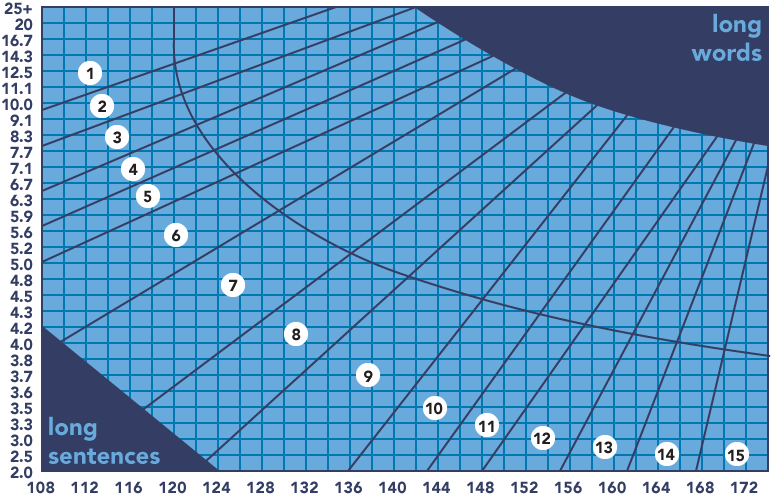
\includegraphics[width=0.8\textwidth]{Bilder/Fry_Graph.png} % Quellenbez.
\caption{An example of a Fry Readability Graph.}
%TODO weil footnote klappt nicht \footnote{Source: \url{http://commons.wikimedia.org/wiki/File:Fry_Graph.png}, accessed on 15.01.2012.}}}
\label{fig:fry_chart}
\end{figure}



\subsection{State of the art approaches to assessing readability}\label{sec:stateof}

Recent approaches are generally still using the ideas as mentioned above. For example Si et al. \cite{Si2001} and Collins-Thompson et al. \cite{Collins-Thompson2004} extend the idea of the word list for assessing the semantic difficulty (which can be viewed as simple language model) to complete unigram language models, which represent the frequency distribution of words in for given texts. They then both use a supervised classification algorithm to classify web sites that where pre-labeled based on expert judgment.

Schwarm and Ostendorf \cite{Schwarm2005}, Feng et al. \cite{Feng2010} and Heilman et al. \cite{Heilman2007} do also use language models, but do as many of the classic formulas also include a measure for syntactic difficulty. They included in addition to the input selected by the word frequencies, also syntactic information obtained by Part-of-Speech tagging - this is the mapping of a labels such as "subject", "object" and "predicate" to the words of a sentence (POS-tagging). This can be represented in a so called parse tree (see figure \ref{fig:parse_tree}).

\begin{figure}
\centering
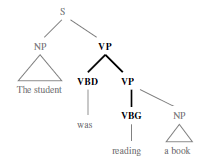
\includegraphics[]{Bilder/parse_tree.png}
\caption{An example parse tree (source: \cite{Heilman2007}).}
\label{fig:parse_tree}
\end{figure}

Other than the above mentioned approaches, Kanungo and Orr \cite{Kanungo2009} did not use a classifier, but a regression model, and focused on a more narrow application: short web summaries. As input for the model they use different values for the semantic difficulty (average characters per word, average syllables per word, percentage of complex words), different features specifically for this task (e.g. Capital Letter Fraction) and even other readability formulas (FOG, Flesch and Flesch-Kincaid).

Kate et al. \cite{Kate2010} use a variety of syntactic, semantic (from different language models: e.g. genre-specific and not genre-specific) and lexical features also using a regression model, and show that the combination of these different kinds of features result in a higher correlation than any of the features on their own.

Xing et al. \cite{Xing2008} further improve the idea of a language model. Instead of using simply a unigram model, they use a bigram model reasoning that the order of words influences the information contained by a sentence and hence influencing readability - e.g. if you reverse a sentence a classical measure such as the Flesch score will not change while you can certainly assume that the sentence is then less readable.

Petersen and Ostendorf \cite{Petersen2006} also combine a variety of features. They extend the language model to n-gram language models, also include POS-parsing information and even classical measures in their model (e.g. Flesch-Kincaid score, average sentence length, average number of syllables per word).

As all the approaches introduced in this section need a big sample of already labeled training data (similar to the criterion passages as discussed with the classical measures), these approaches are out of scope of this paper. This paper will therefore focus on the classical measures, and on the visualization of readability measures. We will provide an approach to enhance the Dale-Chall Measure, as one of the more sophisticated and most accurate classic approaches, and validated it against the other measures (see section \ref{sec:NDC_enhanced}).

\subsection{Visualization of readability} \label{sec:visualization}

Besides measures where the actual method consists of a graphical  visualization such as the Fry Readability Graph, research was e.g. done by Karmakar  and Zhu \cite{Karmakar2010} \cite{Karmakar2010a} in further visualizing readability.
Karmakar and Zhu \cite{Karmakar2010a} propose two different visualizations for numeric readability formulas (they use the Flesch-Kincaid Reading Ease index, the Gunning Fog index, the Coleman-Liau index and the SMOG index), focusing on the comparison of multiple paragraphs of a text to quickly identify sections with low readability:

\begin{itemize}
	\item color coded representation,
	\item and Chernoff faces.
\end{itemize}

For the first they categorized the readability levels into five categories ranging from red (the hardest), to yellow (neutral), to green (the easiest). The readability is then displayed as a colored ring or as a colored string each representing a measure.
The Chernoff faces \cite{Chernoff1973} are cartoon-like faces that can visualize multiple variables with different parts of the face. Here they mapped each readability score to a part of the face (e.g. Flesch-Kincaid mapped to the shape of the faces (circular to oval), ARI is mapped to the orientation of the mouth (smiling to sad), etc.).

Karmakar and Zhu \cite{Karmakar2010} also focus on simplifying the quick visual assessment of the reading difficulty of a text, where differences within the text can easily be spotted. They propose three different visualizations. They base on the classical reading formula components as mentioned above: word complexity (here word length in syllables and letters, and words familiarity as in Dale-Chall) and sentence complexity. Figure \ref{fig:chall_chart} shows an example representation proposed by them. For sentence complexity they do not only use the common metric sentence length, but try to visualize the structural complexity by visualizing the division of clauses in a sentences. The other representation is the visualization of the Dale-Chall Words in a sentence (red not included, grey is included and black is numeric), and also the sentence length. This representation is also implemented in the tool proposed. For an example see section \ref{sec:results}.

\begin{figure}
\centering
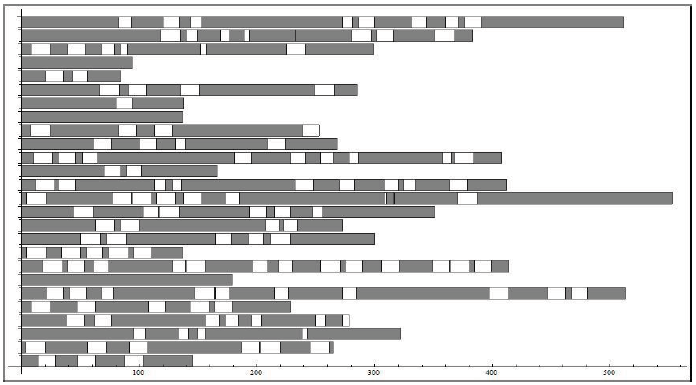
\includegraphics[width=0.8\textwidth]{Bilder/chall_chart.png}
\caption{Visual representation of text complexity (source: \cite{Karmakar2010}).}
\label{fig:chall_chart}
\end{figure}

\section{Method}\label{sec:method}

\subsection{Python, Libraries and Frameworks} \label{sec:method_frameworks}
As the programming language we choose Python because of the existing frameworks, libraries and the ease of use that made the development process modest. As the development environment we used the Enthought Python Distribution (EPD)\footnote{http://enthought.com/products/epd.php} which includes Python 2.7 and over 100 common libraries which are useful for scientific computing. 

We used the following libraries for our Privacy Policy Analyzer:

\begin{itemize}
\item For the visualization respectively the generation of the various charts and diagrams Matplotlib is used.\footnote{\url{http://matplotlib.sourceforge.net/}}
\item NumPy and SciPy provide fundamental functions for scientific computing (e.g. statistics), and provide the array data type which is needed for Matplotlib plots.\footnote{\url{http://numpy.scipy.org/}}
\item We decided to generate our reports with the result of the analytics as simple html files, with a pdf print option. For the template parsing and automated generation of these reports we deployed the python template engine "Cheetah".\footnote{\url{http://www.cheetahtemplate.org/}}
\end{itemize}

Most important is the Natural Language Toolkit (NLTK)\footnote{\url{http://www.nltk.org/}} which provides core features for the analyzer. The NLTK is a framework with capabilities for detailed text analysis and natural language processing. 
For the project we used existing code from the NLTK contribution package, where several readability measures were implemented by students of the University of Agder.\footnote{\url{http://code.google.com/p/nltk/source/browse/trunk/nltk_contrib/nltk_contrib/#nltk_contrib\%2Freadability}}
This existing code already implements a lot of basic measures and syllable, sentence and word counting as well. 

The existence of the NLTK with the readability contribution and the simple handling of lists, string manipulations and general simplicity were the reasons why we decided to build our project on the python programming language.

\subsection{Implementation}\label{sec:implementation}
%Architecture Bild --> verschieden UML-Diagramme (Klassendiagramme, Paketdiagramme, evtl. Use Case Diagramme)
%where did we add s.th. to NLTK_contrib - besonders hervorheben! (e.g. Funktionen nennen)

Figure \ref{fig:diagram} shows a diagram depicting the architecture of the relevant parts of the program "Privacy Policy Analyzer" in an UML-like notation. The parts within the boundaries of the box are all complete novel and created by the authors. Additionally we used, as described above, parts of the Python NLTK contribution package (outside the box), and the NLTK for the enhancement of Dale-Chall. To the code of the contribution package only a few functions where added and minor improvements where done to the code. Table \ref{tab:textanalyzer} shows the added functions.


\begin{table}[htbp]
  \centering
  \caption{Functions added to the existing NTLK contribution source code.}
    \begin{tabular}{p{5cm}p{7cm}}
    \toprule
    \multicolumn{2}{l}{In textanalyzer.py the following functions where added:}  \\
    \midrule
    def countNewDaleChallWordsNotInList & returns the Number of Words not in the original Dale-Chall-List (see section \ref{sec:NDC_enhanced}) \\
    def countNewDaleChallWordsNotInList\_enhanced & returns the Number of Words not in the enhanced Dale-Chall-List (see section \ref{sec:dale_chall}) \\
    \midrule
    \multicolumn{2}{l}{In readabilitytests.py the following functions where added:}  \\
    \midrule
    def NewDaleChall & \multirow{2}[0]{*}{\parbox[t]{7cm}{return the original Dale-Chall score and grade using the above functions}} \\
    def NewDaleChall\_grade &  \\
    def NewDaleChall\_enhanced & \multirow{2}[0]{*}{\parbox[t]{7cm}{return the enhanced Dale-Chall score and grade using the above functions}} \\
    def NewDaleChall\_grade\_enhanced &  \\
    get\_test\_scores & returns the all test scores as a dictionary (before the results where only printed on the console) \\
    \bottomrule
    \end{tabular}%
  \label{tab:textanalyzer}%
\end{table}%


The class \emph{readabilityanalyzer} is the main class used to integrate all parts of the program, and can be used by the user to interact with all functionalities. Alternatively the user can use most functionalities also by using a simple GUI provided by the \emph{input} class. The classes included in the \emph{database} package provide for all functionalities needed to interact with the database storing the texts obtained from the websites. The \emph{presentation} package provides several graphs based on the Matplotlib library for the data provided. The packages \emph{output} and \emph{output\_comparison} include all functionalities needed to produce the HTML reports.

\begin{figure}
\centering
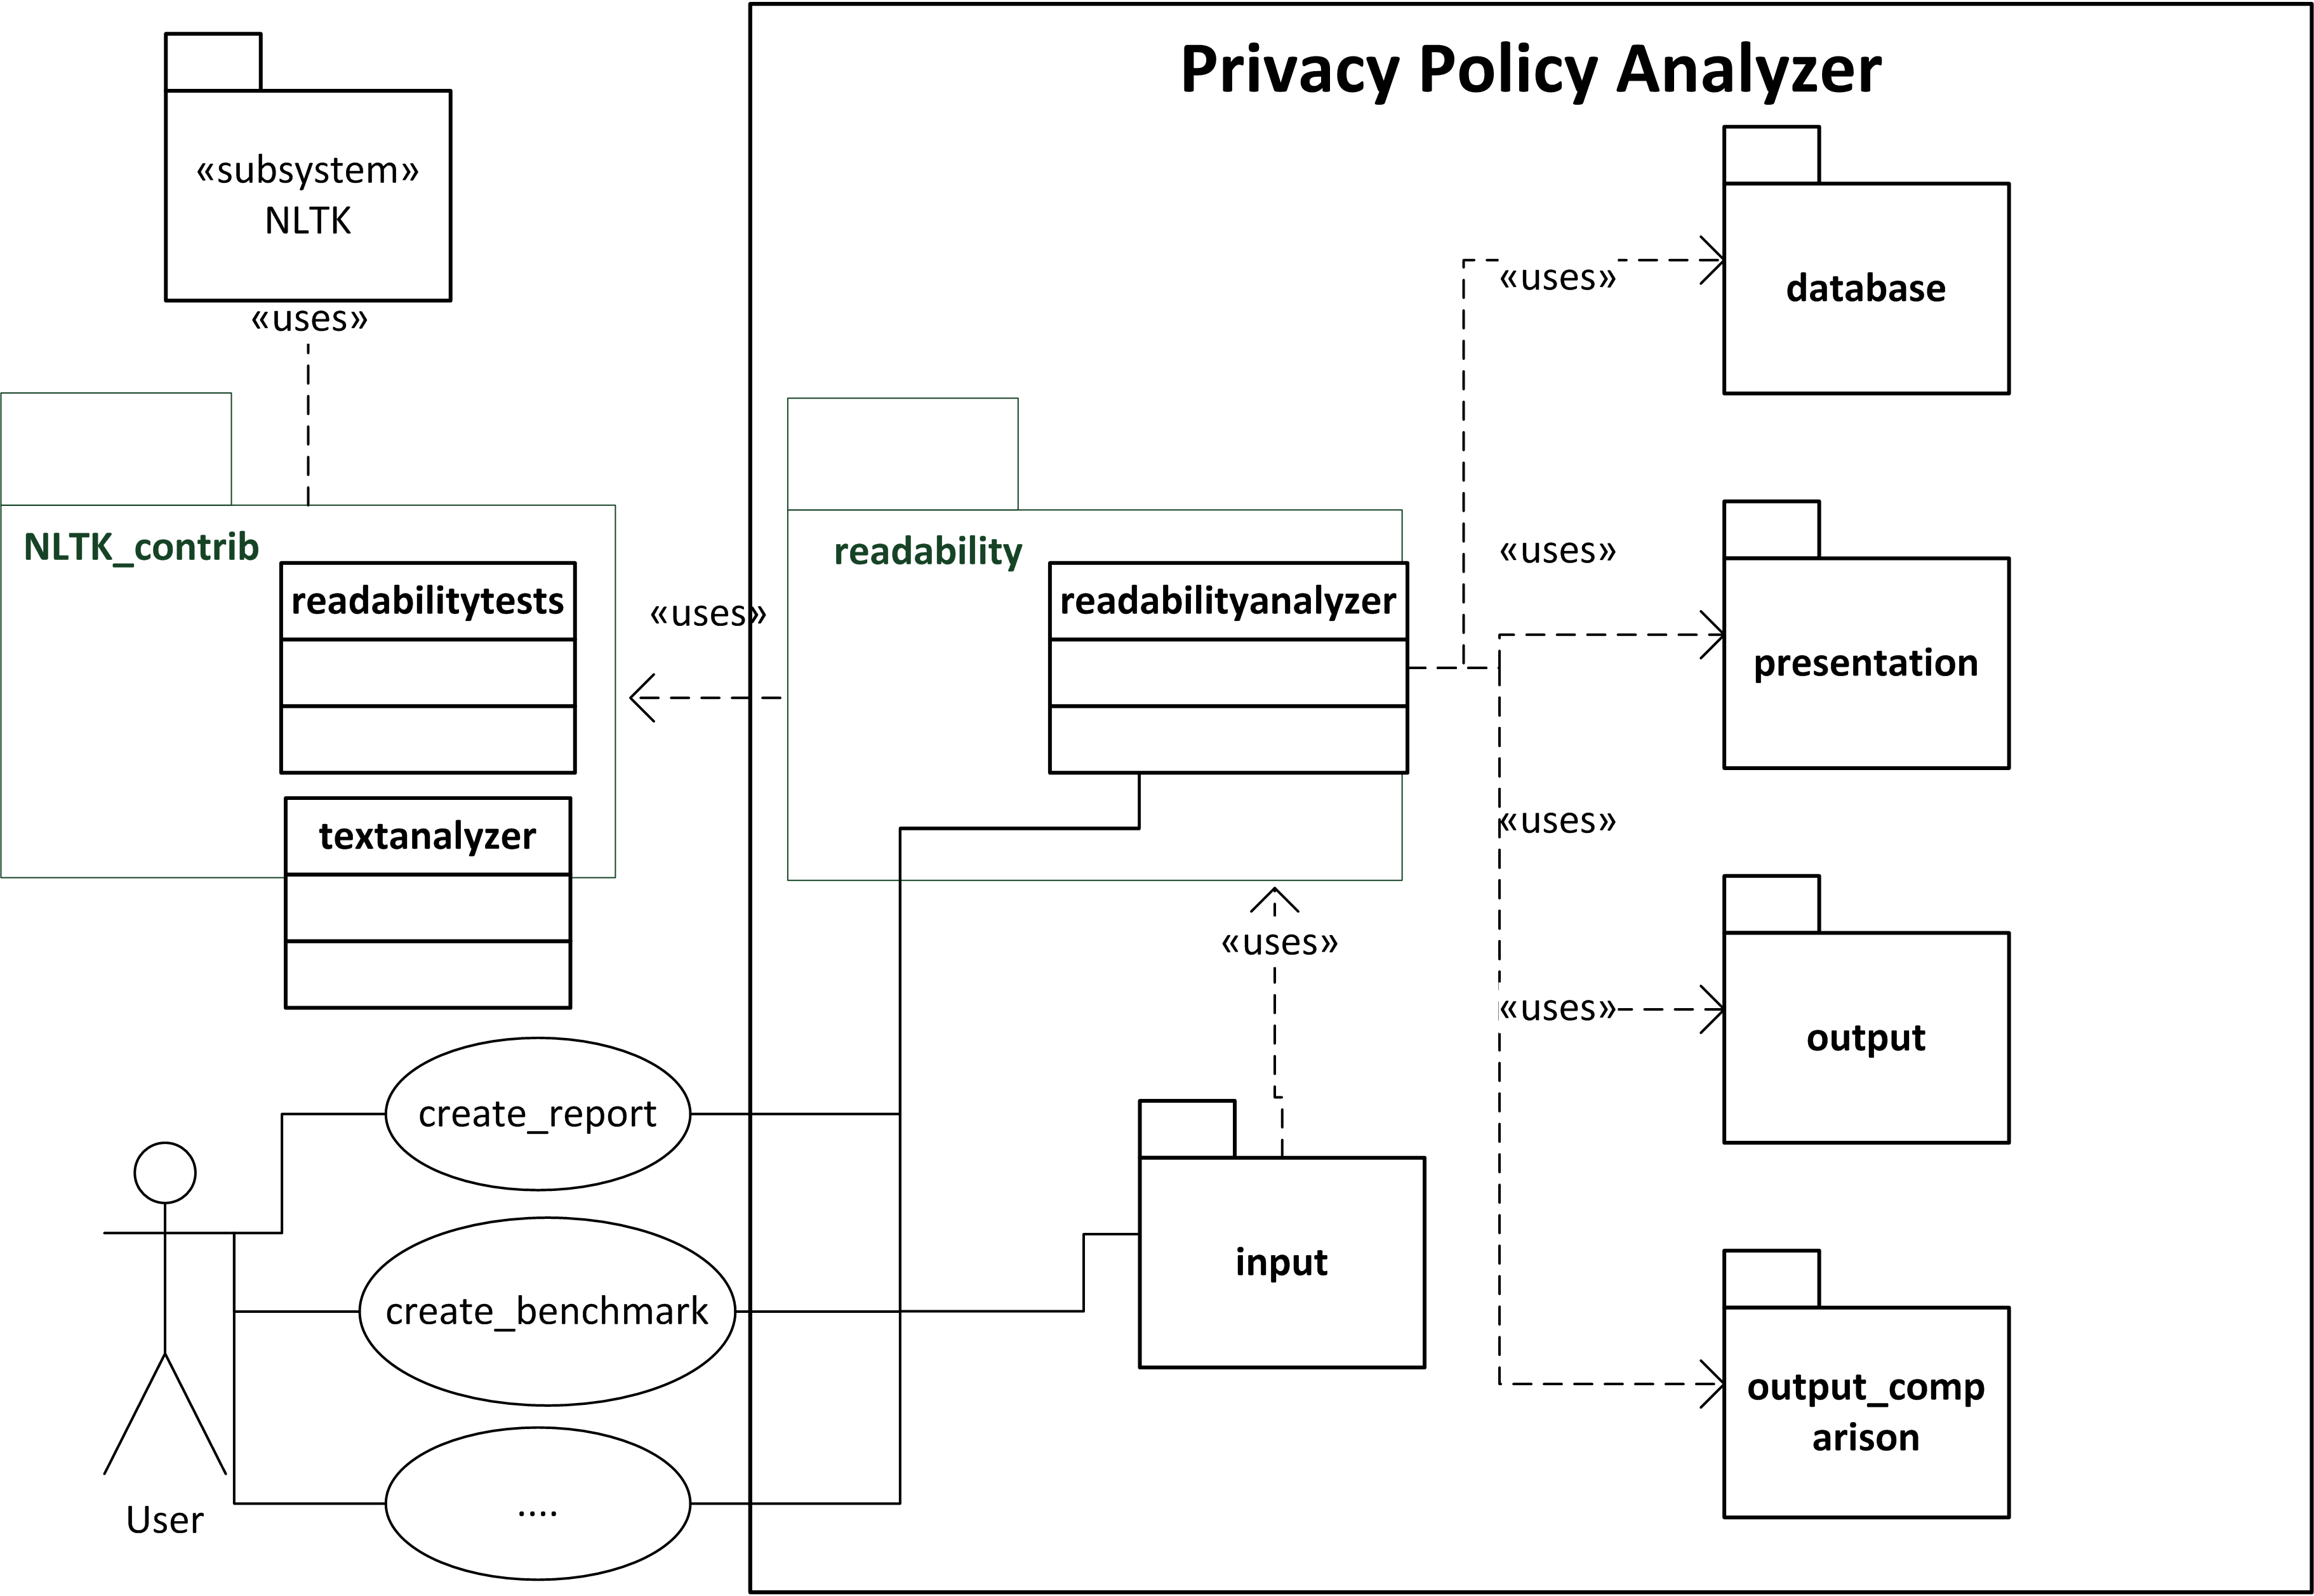
\includegraphics[width=\textwidth]{Bilder/Klassendiagramm.png}
\caption{Architecture of the Privacy Policy Analyzer.}
\label{fig:diagram}
\end{figure}


\subsection{Visualization}\label{sec:visualization}
The reports produced with this work focus much on visualizing readability, to more easily compare the readability among different privacy policies. This is done for one thing with a graphical readability measure (Fry Readability Graph, see section \ref{sec:readability_measures}), a visualization of a classical numeric readability measure (see section \ref{sec:visualization}  as in \cite{Karmakar2010}), and different graphs that simply each visualize different numeric measures for better comparison.

The heat map for example makes it easy to quickly display different numeric measures, and hence compare either different measures for a text, or even see how a measure differs among different texts. It uses a color coding to indicate difficulty, with red being the hardest blending to orange and yellow for medium difficulty and then blending to green as the easiest (see section \ref{fig:heatmap} for an example).

Other plots where implemented, though they are not used in the analysis of this paper. The radar chart is another plot to compare texts, although it is only useful for a smaller amount of texts. A larger area indicates higher scores and therefore a harder readability level. Additional a few statistical plots allow to analyze how the scores for the different measures are distributed among a larger number of texts.


\subsection{Reports}
The tool "Privacy Policy Analyzer" can generate two different reports depending on the objective. In general the reports are automatic generated HTML files which every common browser can display.
The report on the left in figure \ref{fig:reports} shows the results of the analysis of an single privacy policy. It contains some metadata, like name and date of the polices and the original text as well. After the metadata a table with the results of the different measures and the generated visual results are following. The second report on the right hand in figure \ref{fig:reports} is a comparison report, which compares multiple privacy policies against each other. The structure is similar to the single report, including metadata, an overview table of the numeric measure results and some visualizations of the comparison.

\begin{figure}
\centering
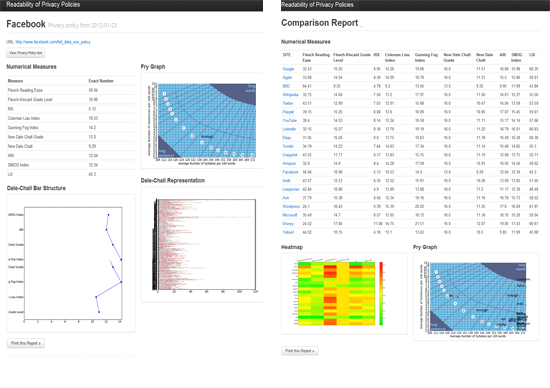
\includegraphics[width=\textwidth]{Bilder/reports2.png}
\caption{Two reports generated by the Privacy Policy Analyze. Left a comparison, right a single report.}
\label{fig:reports}
\end{figure}


\subsection{Adjusting New Dale-Chall Readability index for assessing readability of privacy policies} \label{sec:NDC_enhanced}
The Dale-Chall Readability index is based on the average length of sentences on the one hand and a word list on the other (see \ref{sec:dale_chall}). The word list with 3000 words represents the most \emph{elemental words} in the English language. The Dale-Chall is as mentioned viewed as one of the most accurate classical readability measures. However, when applied to the privacy policies the scores are all extremely high and show just few variability among the privacy policies.

An analysis of the word frequency distribution shows that among the most frequent words (after elimination of all Dale-Chall words) in the privacy policies are on the one hand the names of the corresponding company, and also a set of vocabulary that is frequently used among the policies. Among some of the site's names, some of the most frequent words are e.g. information, personal, services, data or privacy.  These, and the other words, could be considered as essential in order to write a privacy policy. Assuming that you cannot write a privacy policy without a certain set of words it would not to be right to "punish" a site with a bad readability score, when using it. This set of words should be viewed as \emph{elemental words} in a privacy policy, and hence be required as known vocabulary to anybody attempting to read it.

Figure \ref{fig:word_frequency} shows the 80 most frequent words obtained from a sample of 20 of the most popular web sites (see \ref{sec:data}), after deleting the Dale-Chall words. After the deleting procedure about 18,000 words were left. The plot shows the cumulative count of the 80 most frequent words. For this attempt to enhance the measurement we chose a cumulative percentage of 33\% of the words left after deleting the Dale-Chall words. This left a list of 54 words that would for this purpose be added to the Dale-Chall list of words. Hence those 54 words make up about 6,000 of the 18,000 words left. 

\begin{figure}
\centering
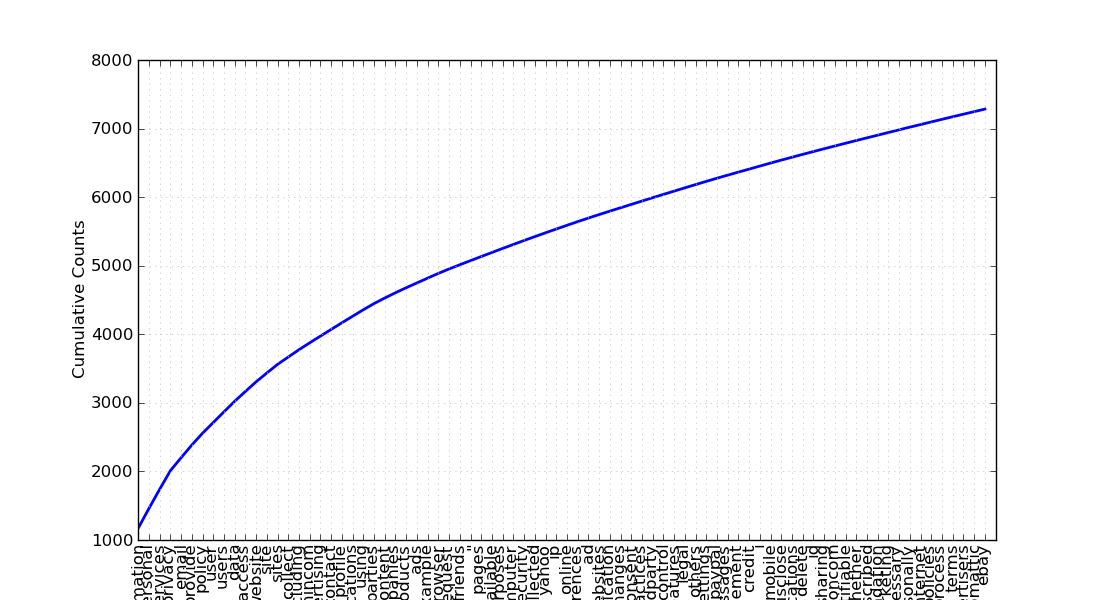
\includegraphics[width=\textwidth]{Bilder/word_frequency_50.png}
\caption{Word frequency for Top 20 privacy policies without Dale-Chall words.}
\label{fig:word_frequency}
\end{figure}

The limitation of this approach of adapting the readability lay in the missing validation through objective assessment of the readability. As discussed in section \ref{sec:readability_measures} this could be done through a study using a comprehension test. This however is out of scope for this paper. An attempt of concurrent validity is given by analyzing correlation with other readability scores in section \ref{sec:validation}.

\subsection{Data}\label{sec:data}

With the goal of having a data basis to analyze, we decided to collect the privacy policies from the most used English websites. As an indicator for most used respectively most visited webpages we relied on the Alexa Web Rank.\footnote{\url{http://www.alexa.com/topsites}} The Alexa Web Rank provides the top websites on a three-month schedule, which is sufficient for our purpose. We collected 20 of the top 50 policies in our database, as metadata we also saved the date, URL and name of the website. Many of the top 50 where left out, as there are many "dublicates" within the top 50 due to different country versions of site, or sites in languages other than English. We decided to use the top 20 web pages because we consider the privacy policy to be more important as the usage of the site increases.

For comparison reasons we decided to add four non privacy policy texts. We added two different classical children's stories. The first one is "A Christmas Tree" written by Charles Dickens \cite{Dickens1988} and the second one is "The Giving Tree" by Shel Silverstein \cite{Silverstein1964}. 
Additionally we added also two old legislative texts, the "Declaration of Independence" from 1776 \cite{decindependence} and the "Bill of Rights" \cite{billofrights} written in 1789.

\section{Results} \label{sec:results}

\subsection{Top 20 Websites}
\begin{figure}
\centering
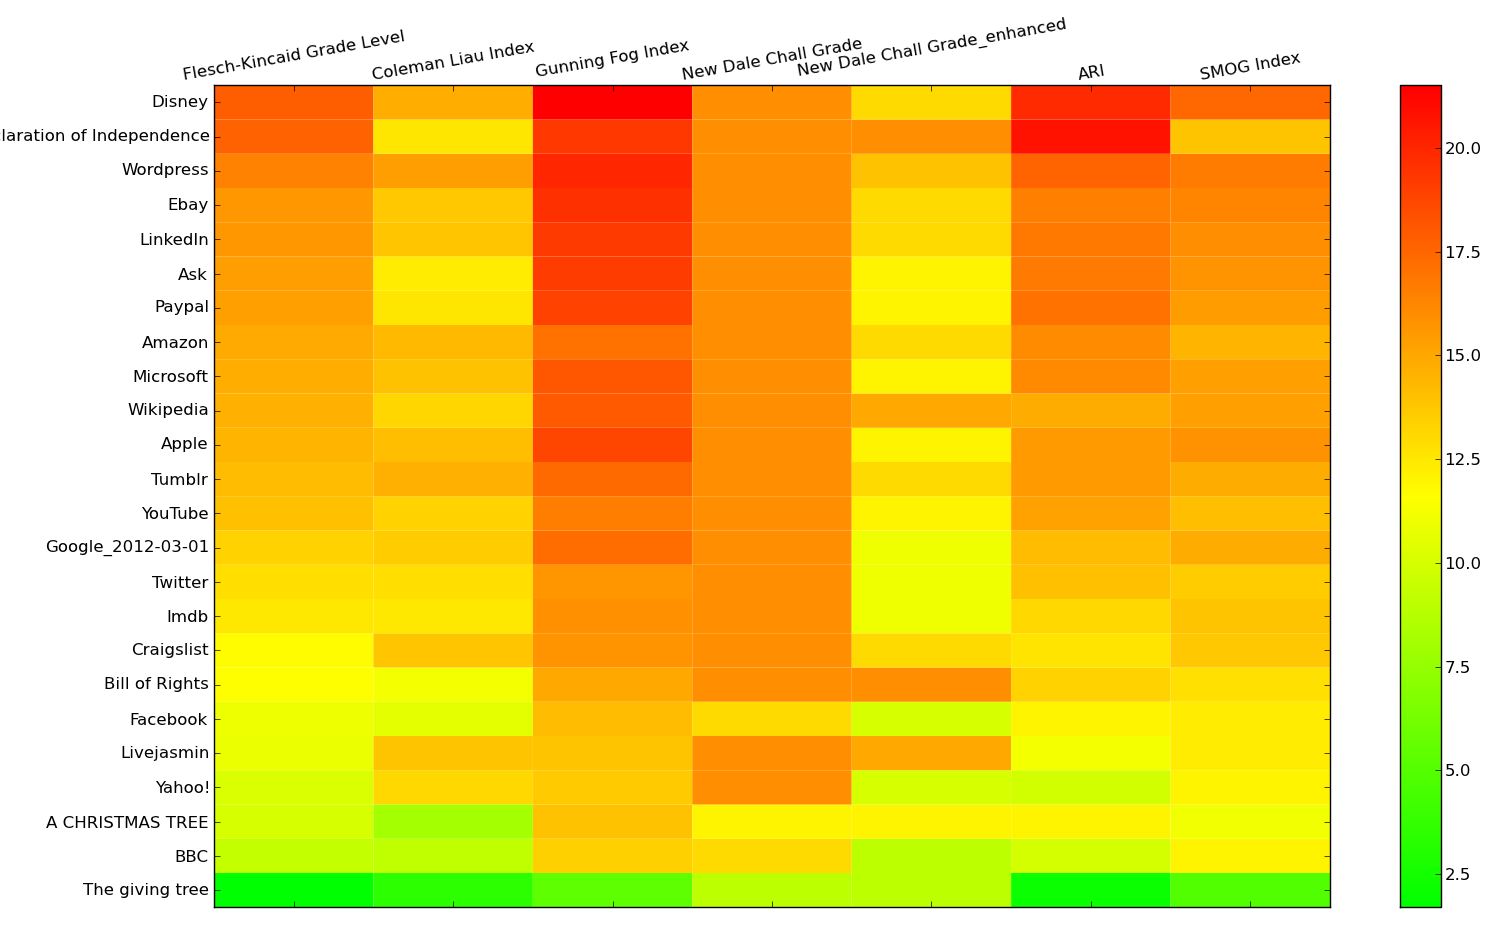
\includegraphics[width=\textwidth]{Bilder/heatmap_alex20_kl.png}
\caption{Heatmap for Top 20 websites}
\label{fig:heatmap}
\end{figure}

The table \ref{tab:allmeasures}, the heat map in figure \ref{fig:heatmap}, the Fry Chart in figure \ref{fig:frytop20} and the Dale-Chall chart in figure \ref{fig:dalechalltop20} show the results of an evaluation with the Privacy Policy Analyzer. The table displays the original numerical results that were obtained and the heat map is provided for a better comparison of the results by visualizing them. The Fry Chart and the Dale-Chall Chart are further visual aids to better compare the readability as mentioned in \ref{sec:visualization}.

%Input data is the collected database with 20 policies from the Top 20 Websites listed by the Alexa Web Rank (as described in \ref{sec:data}). 

\begin{figure}
\centering
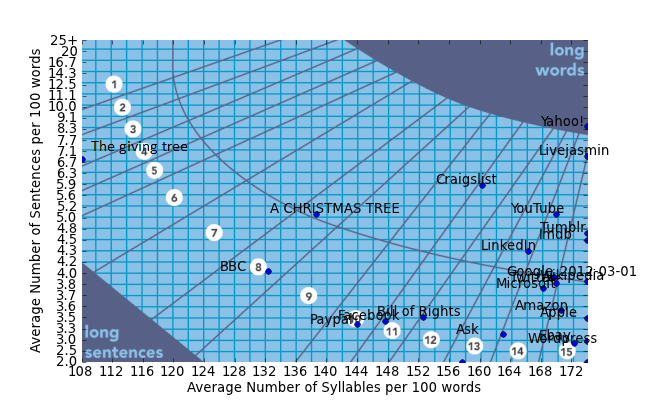
\includegraphics[width=\textwidth]{Bilder/fry_chart_alex20.png}
\caption{Fry Chart with the Top 20 websites and four comparison texts.}
\label{fig:frytop20}
\end{figure}

In the table \ref{tab:allmeasures} the bold marked numbers indicate the simplest text difficulty for each score. Italic marked numbers in contrast indicate the hardest text difficulty for each measure. The fact that the hardest 2 are generally distributed among 2 policies and the worst are distributed among 3 indicates that the scores show some correlation among the various measures. There are however some deviations existent. These are strongest for the Dale-Chall and the enhanced version of the Dale-Chall, but over all one can see that the very easiest, and respectively, the very hardest readable policies and texts stay consistent. For a thorough analysis of the correlation between the measures see section \ref{sec:validation}. The heat map in figure \ref{fig:heatmap} also underpins this relationship described. 




\begin{sidewaystable}[]
  \centering
    \caption{Measure Results for the Top 20 websites}
    \begin{tabular}{p{3.3cm}p{1.5cm}p{1.5cm}p{1.5cm}p{1.5cm}p{1.5cm}p{1.5cm}p{1.5cm}p{1.5cm}p{1.5cm}p{1.5cm}p{1.5cm}p{1.5cm}}
    \toprule
    \textbf{} & \textbf{Flesch Reading Ease} & \textbf{Flesch-Kincaid} & \textbf{RIX} & \textbf{Coleman-Liau} & \textbf{Gunning Fog} & \textbf{New Dale Chall} & \textbf{New Dale Chall Grade} & \textbf{New Dale Chall Score enhanced} & \textbf{New Dale Chall grade enhanced} & \textbf{ARI} & \textbf{SMOG} & \textbf{LIX} \\
    \midrule
    Wordpress & \textit{24.03} & \textit{16.46} & \textit{09.39} & \textit{15.39} & \textit{20.05} & 11.35 & \textit{16} & 09.50 & 14    & \textit{17.60} & \textit{16.71} & \textit{61.97} \\
    Disney & \textit{24.52} & \textit{17.84} & \textit{11.08} & \textit{14.75} & \textit{21.51} & \textit{12.07} & \textit{16} & 09.27 & 13    & \textit{19.85} & \textit{17.43} & \textit{66.61} \\
    Ebay  & 31.05 & 15.58 & 09.00 & 13.75 & 19.63 & 11.39 & \textit{16} & 09.28 & 13    & 16.49 & 16.38 & 60.38 \\
    LinkedIn & 32.15 & 15.57 & 09.16 & 13.79 & 19.19 & 11.22 & \textit{16} & 09.30 & 13    & 16.79 & 16.01 & 60.83 \\
    Amazon & 32.60 & 14.90 & 08.40 & 14.28 & 17.09 & 10.91 & \textit{16} & 09.05 & 13    & 16.05 & 14.54 & 58.62 \\
    Wikipedia & 32.75 & 14.68 & 07.58 & 13.20 & 17.97 & \textit{11.56} & \textit{16} & \textit{09.89} & \textit{15} & 14.81 & 15.27 & 55.56 \\
    Apple & 33.68 & 14.54 & 08.36 & 14.09 & 18.78 & 11.21 & \textit{16} & 08.60 & 12    & 15.50 & 15.86 & 58.81 \\
    Tumblr & 34.19 & 14.22 & 07.44 & 14.63 & 17.34 & 11.14 & \textit{16} & 09.11 & 13    & 15.48 & 14.85 & 55.30 \\
    Microsoft & 35.49 & 14.70 & 08.57 & 13.95 & 18.12 & 11.16 & \textit{16} & 08.94 & 12    & 16.15 & 15.29 & 59.04 \\
    Ask   & 37.79 & 15.38 & 08.56 & 12.34 & 19.16 & 11.16 & \textit{16} & 08.92 & 12    & 16.76 & 15.73 & 58.52 \\
    YouTube & 38.40 & 14.03 & 08.14 & 13.34 & 16.58 & 11.11 & \textit{16} & 08.97 & 12    & 15.17 & 14.14 & 57.66 \\
    Google\_2012-03-01 & 39.05 & 13.32 & 07.13 & 13.57 & 17.28 & 11.00 & \textit{16} & 08.47 & 11    & 14.23 & 14.82 & 54.32 \\
    Paypal & 39.15 & 15.25 & 08.88 & 12.60 & 18.89 & 10.85 & \textit{16} & 08.90 & 12    & 17.07 & 15.45 & 59.61 \\
    Livejasmin & 42.84 & 10.86 & 04.90 & 13.89 & 13.88 & 11.20 & \textit{16} & \textit{09.96} & \textit{15} & 11.17 & 12.36 & 48.48 \\
    Twitter & 43.51 & 12.89 & 07.03 & 12.91 & 15.68 & 10.47 & \textit{16} & 08.37 & 11    & 14.04 & 13.58 & 53.59 \\ref
    Craigslist & 43.55 & 11.71 & 06.17 & 13.83 & 15.75 & 11.19 & \textit{16} & 09.09 & 13    & 12.68 & 13.75 & 52.11 \\
    Imdb  & 43.57 & 12.53 & 06.35 & 12.52 & 15.91 & 10.26 & \textit{16} & 08.27 & 11    & 13.09 & 13.85 & 51.05 \\
    Yahoo! & 44.52 & \textbf{10.15} & \textbf{04.18} & 13.10 & \textbf{13.63} & 10.50 & \textit{16} & 07.92 & \textbf{10} & \textbf{09.85} & \textbf{11.99} & 45.98 \\
    Facebook & \textbf{56.94} & 10.96 & 05.13 & \textbf{10.53} & 14.20 & \textbf{09.29} & \textbf{13} & \textbf{07.70} & \textbf{10} & 12.04 & 12.34 & \textbf{45.30} \\
    BBC   & \textbf{64.41} & \textbf{09.35} & \textbf{04.78} & \textbf{09.20} & \textbf{13.45} & \textbf{09.25} & \textbf{13} & \textbf{07.14} & \textbf{09} & \textbf{09.95} & \textbf{11.99} & \textbf{43.84} \\
\midrule    
    A christmas tree & 71.15 & 10.03 & 04.30 & 08.10 & 13.99 & 08.62 & 12    & 08.65 & 12    & 12.04 & 11.07 & 42.89 \\
    The giving tree & 104.96 & 01.70 & 01.39 & 03.46 & 05.34 & 07.27 & 09    & 07.27 & 09    & 02.11 & 04.88 & 23.63 \\
    Decl. of Independence & 35.31 & 17.70 & 09.97 & 12.56 & 19.30 & 10.71 & 16    & 10.84 & 16    & 20.75 & 13.92 & 64.15 \\
    Bill of Rights & 55.25 & 11.62 & 06.37 & 11.18 & 14.97 & 10.25 & 16    & 10.31 & 16    & 13.33 & 12.77 & 50.51 \\
    \bottomrule
    \end{tabular}%
  \label{tab:allmeasures}%
\end{sidewaystable}%

Both the table and the heat map show that Wordpress.com and Disney.com consistently are the hardest-to-read policies from our database. 
The best results for readability of their privacy policies have the websites Yahoo.com, Facebook.com and BBC.co.uk. At least for BBC.co.uk and Facebook.com the Fry Charts support their good readability score (see figure \ref{fig:frytop20}). For Yahoo.com the Fry Chart shows that the policy contains short sentences but long words. This fact is also displayed in the Dale-Chall representation of Yahoo.com in figure \ref{fig:dalechalltop20}, where it is compared to Disney.com, as one of the hardest sites, and two of the comparison texts. Here one can see that it has considerably shorter sentences as Disney.com. It shows however, that it is still a lot more difficult than the children's story "The giving tree".

The heat map and the Fry Chart also very clearly show that the children's stories stand out in comparison even with the easiest policies. The "Declaration of Independence" in contrast scores among the most difficult texts analyzed.

Generally the analysis shows that for almost every policy the scores result in grade levels (Flesch-Kincaid, Coleman-Liau, Gunning Fog, New Dale Chall, ARI, SMOG) of 13 and higher, which means that a reading capability at college level is required to comfortably read these privacy policies.

\begin{figure}
\centering
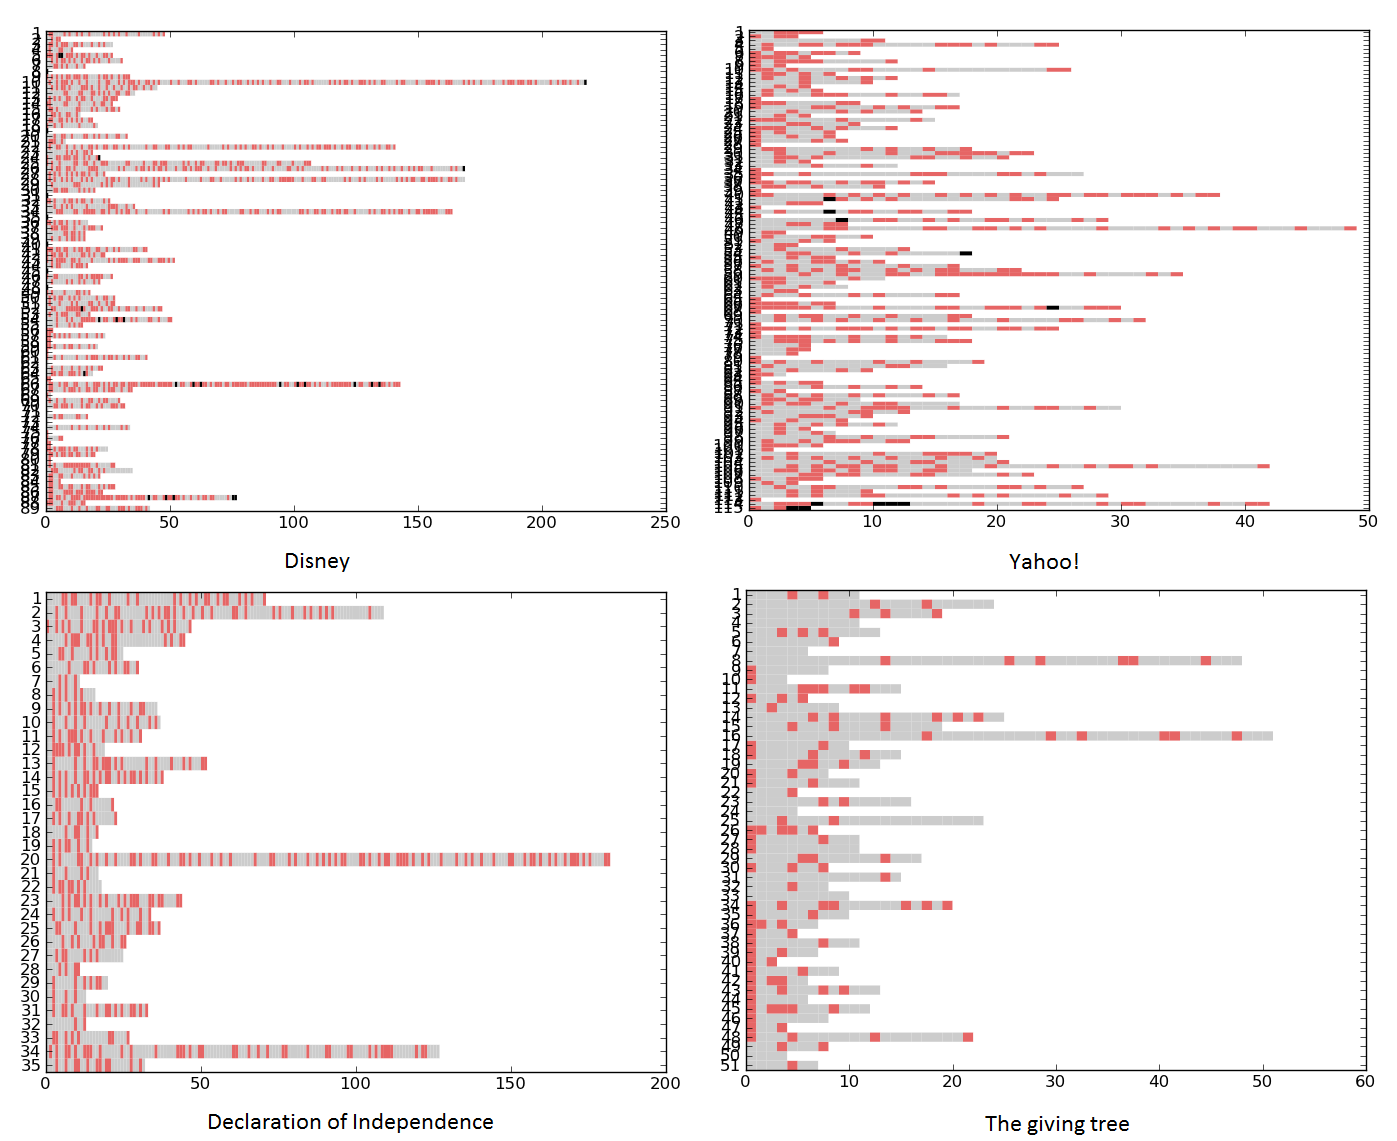
\includegraphics[width=\textwidth]{Bilder/dalechall_comparison.png}
\caption{Dale Chall Chart for four texts.}
\label{fig:dalechalltop20}
\end{figure}

\subsection{Google privacy policy over time}
\begin{table}%[h!]
  \centering
  \caption{Google privacy policies over time scores.}
    \begin{tabular}{p{1.8cm}p{1cm}p{1.3cm}p{1.5cm}p{1.1cm}p{1cm}p{1cm}p{1cm}p{1cm}}
    \toprule
    \multicolumn{1}{c}{\parbox[t]{1.8cm}{\textbf{Date of\\ Policy}}} & \multicolumn{1}{c}{\parbox[t]{1.3cm}{\textbf{Flesch \\Kincaid}}} & \multicolumn{1}{c}{\parbox[t]{1.3cm}{\textbf{Coleman\\Liau}}} & \multicolumn{1}{c}{\parbox[t]{1.3cm}{\textbf{Gunning\\ Fog}}} & \multicolumn{1}{c}{\parbox[t]{1.1cm}{\textbf{NDC \\Score enh.}}} & \multicolumn{1}{c}{\textbf{NDC}} & \multicolumn{1}{c}{\parbox[t]{1cm}{\textbf{NDC \\Grade enh.}}} & \multicolumn{1}{c}{\textbf{ARI}} & \textbf{SMOG} \\
    \midrule
    2000-08-14 & 11,15 & 11,44 & 13,69 & 8,48  & 10,42 & 11    & 12,01 & 12,12 \\
    2004-07-01 & 12,23 & 12,74 & 16,51 & 8,1   & 10,29 & 11    & 12,93 & 14,3 \\
    2005-10-14 & 15,79 & 13,97 & 19,99 & 8,96  & 11,49 & 12    & 17,13 & 16,6 \\
    2008-08-07 & 15,81 & 14,08 & 19,97 & 8,92  & 11,59 & 12    & 17,05 & 16,6 \\
    2009-01-27 & 15,71 & 14,06 & 19,82 & 8,89  & 11,56 & 12    & 16,92 & 16,51 \\
    2009-03-11 & 16,02 & 14,21 & 20,18 & 8,96  & 11,67 & 12    & 17,32 & 16,75 \\
    2010-10-03 & 15,31 & 14,21 & 19,11 & 9,01  & 11,53 & 13    & 16,63 & 16,02 \\
    2011-10-20 & 15,25 & 14,26 & 19,06 & 9,04  & 11,51 & 13    & 16,66 & 15,98 \\
    2012-03-01 & 13,32 & 13,57 & 17,28 & 8,47  & 11    & 11    & 14,23 & 14,82 \\
    \bottomrule
    \end{tabular}
  \label{tab:google}%
\end{table}%

\begin{figure}
\centering
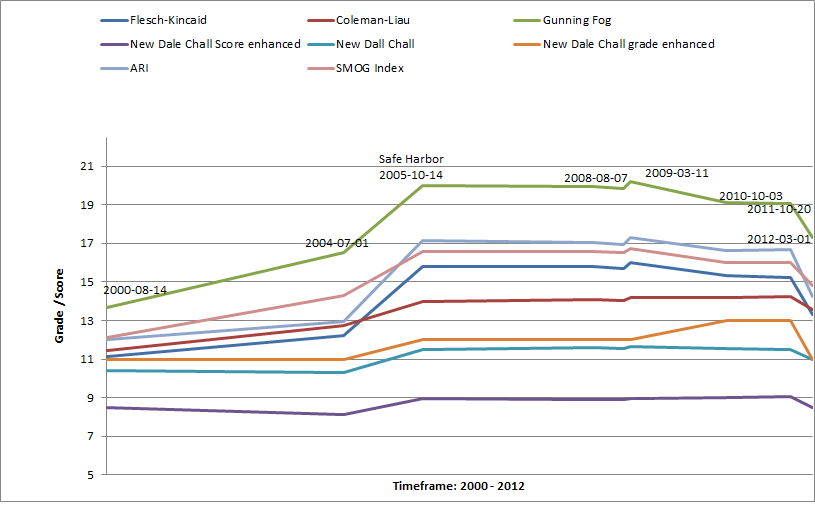
\includegraphics[width=\textwidth]{Bilder/google_over_time_diagram.png}
\caption{Readability of Google Privacy Policies over Time. Based on data of table \ref{tab:google}.}
\label{fig:google_over_time_diagram}
\end{figure}
In the previous section we could only analyze a snapshot of the current privacy policies of the websites. As Sumeeth et al. \cite{Sumeeth2010} we were also interested in how privacy policies developed over time. Google provides an archive of their privacy policy since August 2000.\footnote{http://www.google.com/intl/en/policies/privacy/archive/} Since Google is currently the most popular web site we want to provide a thorough analysis of the readability of their privacy policy. They state that they want to be transparent as possible regarding changes. We used this possibility to compile a comparison report on the English version of the Google privacy policy to analyze changes over time with the Privacy Policy Analyzer. The input data for the analysis are nine different versions starting in 2000 until 2012 (as seen in table \ref{tab:google}). Results are the various measures that our tool provides and visual representation through the Fry Graph in figure \ref{fig:google_over_time}.

As one can see in the plot in figure \ref{fig:google_over_time_diagram} and the Fry Graph in figure \ref{fig:google_over_time} the privacy policy was relatively readable when starting in 2000. Table \ref{tab:google} provides the numbers used in figure \ref{fig:google_over_time_diagram}. In the time frame from 2000 to 2004 no changes were applied as opposed to the time after 2008 where the policy changed at least once a year. With the changes in 2004 and 2005 one can see a clear increase in the difficulty of readability. This level stays with small changes until the second change of the policy in 2009 (2009-03-11), where the peak of all measures except New Dale Chall is reached. After this peak level the readability gets easier with almost every change to the policy. 
The last update from 2012-03-01 had among the consolidation of many policies also the scope to improve the readability, as Google stated \cite{Google2012}. Expressed in readability measures a visible improvement in comparison to the previous versions exists, but it is still slightly more difficult than the 2004 version and the 2000 version anyway.
One possible reason for the significant jump between 2004 and 2005 could be the fact that Google joined the U.S.-EU Safe Harbor Act in 2005 \cite{safeharbor}. For the Safe Harbor certification a comprehensive and detailed privacy policy is mandatory \cite{safeharbor2}. Based on the limitations of this paper, the dependences between changes in the Google policy and the Safe Harbor certification are not further investigated.

The Google over time analysis also indicated the correlation between the different measures. Though they do not result in equal numeric results, they generally are all indicating the same leaps triggered by changes in the privacy policy text. The line chart gives a good visualization of this. For a deeper analysis regarding statistical correlation in general between the readability measures see section \ref{sec:validation}.

\begin{figure}
\centering
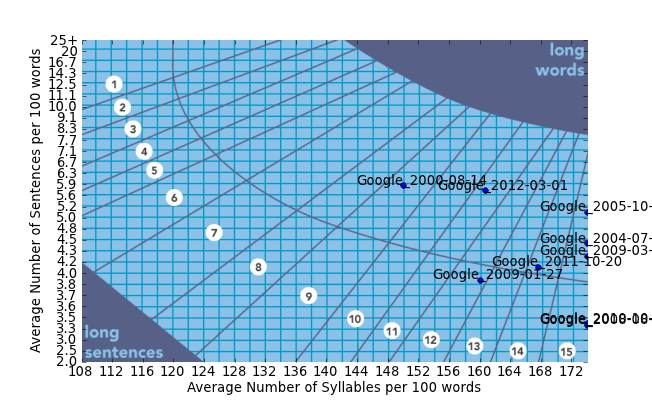
\includegraphics[width=\textwidth]{Bilder/google_over_time.png}
\caption{Readability of Google Privacy Policies over Time.}
\label{fig:google_over_time}
\end{figure}


\subsection{Validation of method}\label{sec:validation}

In this section we want to reflect on the method used. We want to verify the implementation of the readability measures on the one side and attempt to verify the adjustment of the Dale-Chall measure as discussed in section \ref{sec:NDC_enhanced}. As discussed in section \ref{sec:readability_measures} there are generally three widely used approaches to verify readability measures: correlation with the score of reading comprehension tests, the score of expert judgements or other readability scores. As the first two are out of the scope of this paper we will use the latter by analyzing the correlation between the implemented measures. 

Table \ref{tab:correlation} shows the Pearson correlation coefficients between the measures discussed in this paper and implemented the Readability Analyzer (exceptions are the visual measures such as the Fry Chart). The scores are based on the application to the 20 privacy policies and four "benchmark" texts as discussed in section \ref{sec:data}. It shows that all coefficients are statistically significant at the 5\% significance level (most even at the 1\% level).

It shows that all the scores that are based on solely easier syntactic features, and word length as a semantic feature, correlate highly with coefficients of more than 0,8 and many even higher than 0,9. All correlate positively except with Flesch Reading Ease, as this score decreases as a text becomes more difficult as opposed to all the other scores. From those measures Coleman-Liau correlates the weakest with the other scores. Also the New-Dale Chall score with the word list as a semantic part (and its obtained grade) does correlate pretty highly with the other scores. The "enhanced" version however does not correlate much with the scores, with only low coefficients around 0,5 - 0,6. This much limits it's \emph{objective} validity to measure the readability of Privacy Policies. To validate it further, therefore other objective approaches are needed to validate its applicability objectively.

\begin{sidewaystable}[]
  \centering
  \caption{Pearson correlation coefficients for readability measures, where * indicates p-value of 5\%, and ** indicates a p-value of 1\%}
    \begin{tabular}{p{3cm}p{1.1cm}p{1.2cm}p{1.5cm}p{1.4cm}p{1.1cm}p{1.1cm}p{1.1cm}p{1.1cm}p{1.1cm}p{1.1cm}p{1.1cm}p{1.1cm}}
    \toprule
          & \textbf{Flesch Reading Ease} & \textbf{Flesch-Kincaid} & \textbf{Coleman-Liau} & \textbf{Gunning Fog} & \textbf{ARI} & \textbf{SMOG} & \textbf{LIX} & \textbf{RIX} & \textbf{NDC} & \textbf{NDC grade} & \textbf{NDC enhanced} & \textbf{NDC grade enhanced} \\
    \midrule
    Flesch Reading Ease & 1     & -,930** & -,969** & -,922** & -,868** & -,949** & -,942** & -,865** & -,958** & -,919** & -,563** & -,508* \\
    Flesch-Kincaid & -,930** & 1     & ,830** & ,983** & ,987** & ,944** & ,990** & ,965** & ,854** & ,807** & ,630** & ,557** \\
    Coleman-Liau & -,969** & ,830** & 1     & ,823** & ,757** & ,882** & ,859** & ,752** & ,950** & ,934** & ,521** & ,480* \\
    Gunning Fog & -,922** & ,983** & ,823** & 1     & ,963** & ,976** & ,977** & ,953** & ,860** & ,789** & ,566** & ,499* \\
    ARI   & -,868** & ,987** & ,757** & ,963** & 1     & ,897** & ,973** & ,965** & ,785** & ,744** & ,653** & ,576** \\
    SMOG  & -,949** & ,944** & ,882** & ,976** & ,897** & 1     & ,950** & ,907** & ,903** & ,834** & ,484* & ,432* \\
    LIX   & -,942** & ,990** & ,859** & ,977** & ,973** & ,950** & 1     & ,973** & ,889** & ,841** & ,625** & ,550** \\
    RIX   & -,865** & ,965** & ,752** & ,953** & ,965** & ,907** & ,973** & 1     & ,812** & ,726** & ,591** & ,512* \\
    NDC   & -,958** & ,854** & ,950** & ,860** & ,785** & ,903** & ,889** & ,812** & 1     & ,924** & ,605** & ,555** \\
    NDC grade & -,919** & ,807** & ,934** & ,789** & ,744** & ,834** & ,841** & ,726** & ,924** & 1     & ,599** & ,544** \\
    NDC enhanced & -,563** & ,630** & ,521** & ,566** & ,653** & ,484* & ,625** & ,591** & ,605** & ,599** & 1     & ,983** \\
    NDC grade enhanced & -,508* & ,557** & ,480* & ,499* & ,576** & ,432* & ,550** & ,512* & ,555** & ,544** & ,983** & 1 \\
    \bottomrule
    \end{tabular}%
  \label{tab:correlation}%
\end{sidewaystable}%

%\multicolumn{13}{l}{**. Correlation is significant at the 0.01 level (2-tailed).}                     & \\
 %\multicolumn{13}{l}{*. Correlation is significant at the 0.05 level (2-tailed).}                      & \\
\section{Conclusion}\label{sec:conclusion}

\subsection{Research limitations}%Ausreichend?
Due to the comprehensive aspects of research regarding readability of privacy policies some research limitations are existent. 
One very important component in any context with privacy policies are the legal aspects. We do not include any part of regulation and legislation into this paper because this is not in our scope. Another limitation are the state-of-the-art measures, which are not part of the Privacy Policy Analyzer, due to the fact that the training of the measures needs a big amount of pre-labeled data. A further limitation in this paper is the quality and quantity of privacy policies in our database. This state of the database is sufficient for the scope of this paper, but could be improved for further research, by collecting more policies.

\subsection{Future Work}
Most of the limitations provide interesting opportunities for future research efforts. Therefore we would suggest the following aspects for further investigation. 
There a some possibilities to improve on the topic readability of privacy policies by using our already developed tool Privacy Policy Analyzer. One could do a more sophisticated analysis with more statistical valid quantitative comparisons using a larger database of policies (e.g. number of policies $>$ 100). The collection of a high number of privacy policies was out of scope of this paper, as insuring sufficient data quality is quite time consuming. 
One aspect which is not noted in this paper is the possibility to expand readability analytics with the way how a policy is presented, like how easy they are to find, which font and font-size on which background color is used etc.
The legal aspects discussed above can be assumed to influence the readability of the privacy policies. The readability measures are usually aimed at grading texts at school level. Hence future work should focus on adjusting them to suit the task of rating privacy policies better. We provided one approach in adjusting the Dale-Chall word list in \ref{sec:NDC_enhanced}. Future research could focus on using approaches similar to those discussed in the section \ref{sec:stateof}. Those require an empirical classification of the readability of the texts e.g. with surveys where privacy policies are manually rated. These results could then be used as training data for the state-of-the-art measures which can then produce results better suited for this specific task.
 
\subsection{Findings} 

In this paper we developed the tool Privacy Policy Analyzer, which can analyze privacy policies based on different measures for text difficulty.
We showed that the readability level of the most privacy policies from popular websites is at college level or above. In coherence with the average age of the internet user and their education one essential statement is, that in general privacy policies compared to the reading comprehension level of the internet user are to difficult. An improvement of readability is necessary to cover most internet users and give them a chance of understanding privacy policies easily. Using Google as an example we show that an improvement of readability can be achieved.

\bibliography{paper}

\end{document}